%----------------------------------------------------------------------------------------
%    PACKAGES AND THEMES
%----------------------------------------------------------------------------------------
\documentclass[aspectratio=169,xcolor=dvipsnames]{beamer}
\makeatletter
\def\input@path{{theme/}}
\makeatother
\usetheme{CleanEasy}
\usepackage[utf8]{inputenc}
\usepackage{lmodern}
\usepackage[T1]{fontenc}
% \usepackage[brazil]{babel}
\usepackage{fix-cm}
\usepackage{amsmath}
\usepackage{mathtools}
\usepackage{listings}
\usepackage{xcolor}
\usepackage{hyperref}
\usepackage{graphicx} % Allows including images
\usepackage{booktabs} % Allows the use of \toprule, \midrule and \bottomrule in tables
\usepackage{tikz}
\usetikzlibrary{positioning, shapes, arrows, calc, decorations.pathreplacing, arrows.meta, backgrounds, patterns, overlay-beamer-styles}
\usepackage{etoolbox}
\usepackage{animate}
\usepackage{svg}

\usepackage[portuguese]{babel}

\graphicspath{ {./Figuras/} }

%----------------------------------------------------------------------------------------
%    LAYOUT CONFIGURATION
%----------------------------------------------------------------------------------------



% Configure code listings
\lstset{
  basicstyle=\ttfamily\small,
  keywordstyle=\color{blue},
  commentstyle=\color{green!60!black},
  stringstyle=\color{red},
  showstringspaces=false,
  breaklines=true,
  frame=single,
  rulecolor=\color{black!30},
  backgroundcolor=\color{black!5},
  numbers=left,
  numberstyle=\tiny\color{black!70},
  numbersep=5pt
}

%----------------------------------------------------------------------------------------
%    TITLE PAGE
%----------------------------------------------------------------------------------------


%---------------------------------------------


\title{Plataformas IoT}

\author[A. Rodrigues]{Arthur H. D. Rodrigues}

\institute[VFU]{
  Mestre em Ciência da Computação\\
  IME - USP
}


\vspace{-2cm}\date{30 de Junho de 2025}
% Define positions for logos on title page


%----------------------------------------------------------------------------------------


\begin{document}

\begin{frame}[plain]
  \titlepage
\end{frame}

\begin{frame}[plain]

\begin{figure}
    \centering
    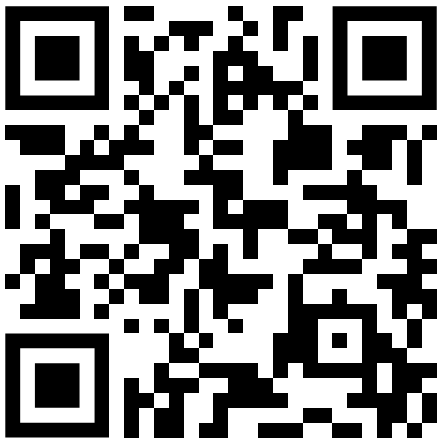
\includegraphics[width=0.5\linewidth]{QR-code-aula-mestrado.png}
    \caption{https://github.com/arthuript/Aula-plataformas-IoT}
\end{figure}
\end{frame}


\begin{frame}[plain]{Contents}
  \tableofcontents
\end{frame}

\section{Arquitetura Geral de Sistemas IoT}
\begin{frame}{Arquitetura em Camadas da IoT}
\begin{figure}
    \centering
 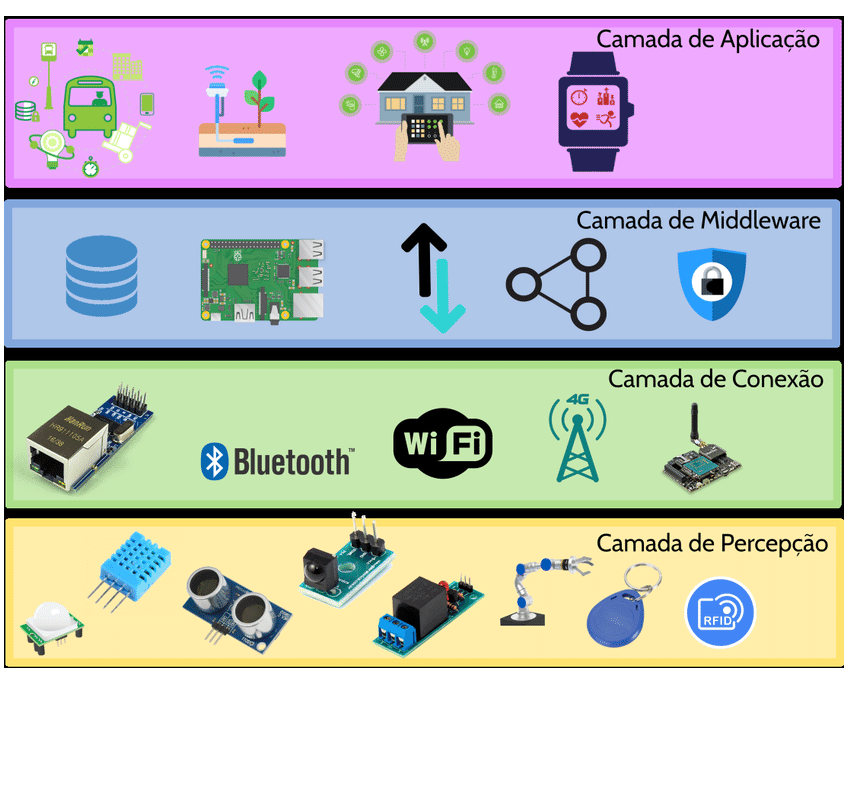
\includegraphics[scale=.32]{Representacao-de-camadas-da-arquitetura-IoT-Adaptado-de-Andrade-et-al-2018}
\end{figure}

  Key features:
  \begin{itemize}
    \item Dispositivos (sensores/atuadores)
    \item Gateways
    \item Redes de comunicação
    \item Plataformas IoT
    \item Aplicações
  \end{itemize}
\end{frame}

\begin{frame}{Camada de middleware}
\begin{exampleblock}{Resumidamente...}
    \begin{itemize}
        \item Software intermediário
        \item "Cola" que liga diferentes componentes num sistema  
        \item Abstrai a complexidade dos dispositivos e da rede
        \item Intermedia a comunicação entre os dispositivos e as aplicações
        \item Gerencia dados, dispositivos, serviços e eventos
    \end{itemize}
    \end{exampleblock} 
    \end{frame}

\begin{frame}{Camada de middleware}
    \begin{exampleblock}{Responsabilidades}
    \begin{itemize}
   \item \textbf{Gerenciamento de dispositivos:}	Cadastro, autenticação, status
    \item    \textbf{Comunicação:}	Interpretação de protocolos (MQTT, CoAP, HTTP...)
    \item    \textbf{Armazenamento intermediário:}	Buffer de dados ou cache
    \item    \textbf{Regras e automações:}	Lógica de eventos ("se temperatura > 30, enviar alerta")
    \item    \textbf{APIs:}	Interface para as aplicações consumirem os dados
     \item   \textbf{Segurança:}	Controle de acesso, autenticação, criptografia
    \end{itemize}
        \end{exampleblock} 
\end{frame}

\begin{frame}{Camada de aplicação}

    \begin{exampleblock}{Responsabilidades}
    \begin{itemize}
    \item \textbf{Visualização de dados:}	Exibe informações coletadas em gráficos, tabelas, mapas etc. Permite interpretar tendências, valores atuais e históricos.
\item \textbf{Interação com o usuário:}	Interfaces Web/Mobile para que o usuário possa visualizar dados, configurar alertas, interagir com dispositivos.
\item \textbf{Dashboard personalizável:} Criação de painéis de controle com widgets (gráficos, gauges, mapas, botões) para representar o sistema.
    \end{itemize}
    \end{exampleblock} 
    \pause
      \begin{alertblock}{Dica}
A camada de aplicação é voltada para o ser humano, enquanto a de middleware é mais voltada para o sistema.
  \end{alertblock}
\end{frame}

\begin{frame}{Camada de plataforma}
\begin{exampleblock}{Plataforma Aplicacional}
\textbf{Plataforma Aplicacional} = camada de middleware + camada de aplicação
\end{exampleblock}
\begin{figure}
    \centering
 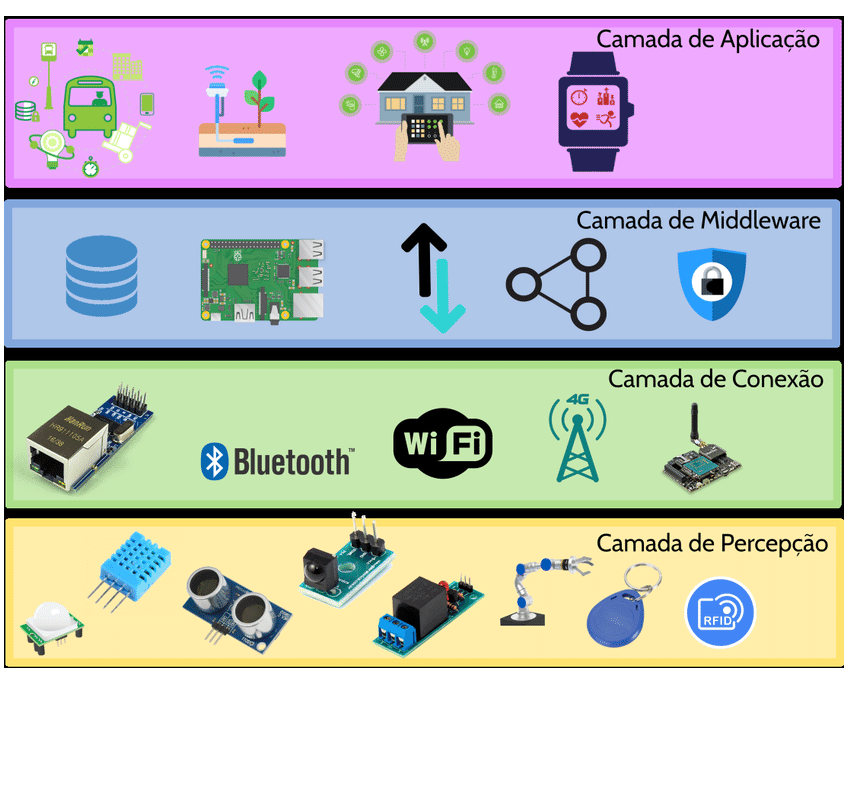
\includegraphics[scale=.33]{Representacao-de-camadas-da-arquitetura-IoT-Adaptado-de-Andrade-et-al-2018}
\end{figure}
\end{frame}

\section{Plataformas IoT: Conceito e Função}

\begin{frame}{O que é uma Plataforma IoT?}
\begin{itemize}
    \item É o ambiente digital que conecta dispositivos IoT à internet e aos usuários
    \item Gerencia dados, dispositivos, usuários e integrações
    \item Atua como ponte entre o mundo físico e usuários
\end{itemize}
\begin{alertblock}{Plataforma Aplicacional}
\textbf{Plataforma Aplicacional} = camada de middleware + camada de aplicação
\end{alertblock}
\end{frame}

\begin{frame}{A importância da Plataforma}
\begin{itemize}
    \item Centraliza comunicação entre milhares de dispositivos
    \item Armazena e processa dados em tempo real
    \item Permite visualização e controle remoto
    \item Garante segurança, escalabilidade e integração
\end{itemize}
\begin{alertblock}{Plataforma}
Sem plataforma, IoT é um monte de sensores isolados. É ela quem dá inteligência ao sistema.\end{alertblock}
\end{frame}

\begin{frame}{Componentes Internos de uma Plataforma}
\begin{itemize}
    \item Broker de mensagens (MQTT, AMQP…)
    \item Banco de dados (TSDB, NoSQL, SQL)
    \item Engine de regras
    \item Módulo de visualização
    \item Gerenciador de dispositivos
    \item APIs REST/WebSocket
\end{itemize}
\end{frame}

\section{Exemplos de Plataformas IoT}

\begin{frame}{Tipos de Plataformas IoT}

\begin{table}[]
    \centering
    \begin{tabular}{|c|c|}
    \hline
       Tipo  & Exemplo  \\
       \hline
       Open Source	  & Ibirapitanga, Interscity, ThingsBoard, Kaa, FIWARE\\
       \hline
       Cloud Proprietária	& AWS IoT, Azure IoT Hub\\
       \hline
    \end{tabular}
\end{table}
\begin{figure}
    \centering
    
\includegraphics[width=0.3\linewidth]{Figuras/logo-ibira.png}
    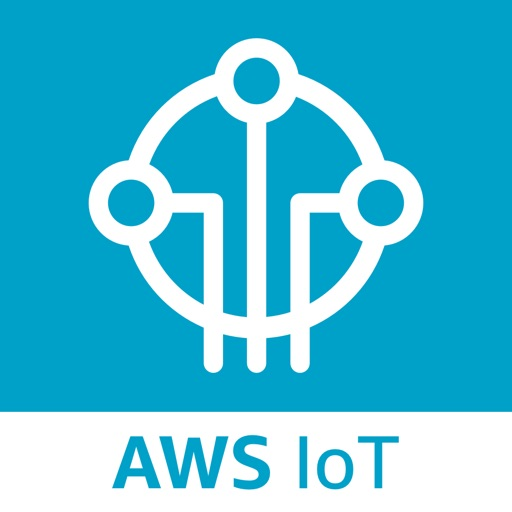
\includegraphics[width=0.3\linewidth]{Figuras/aws-iot.jpg}
\end{figure}
\end{frame}

\section{Ibirapitanga}
\begin{frame}{Ibirapitanga}
  \begin{columns}
    \begin{column}{0.48\textwidth}
    \centering
    
\includegraphics[width=.8\linewidth]{Figuras/logo-ibira.png}
    \end{column}
    \begin{column}{0.48\textwidth}
    \begin{itemize}
        \item Desenvolvida pelo IPT
        \item No do Pau Brasil em tupi
        \item Middleware + aplicação
        \item Microsserviços
        \item Código aberto*
    \end{itemize}
    \end{column}
  \end{columns}
\end{frame}

\begin{frame}{Abstrações básicas}
\begin{itemize}
    \item \textbf{Capabilities:} Tipos de dados coletados:
    \begin{itemize}
        \item Temperatura
        \item Pressão
        \item Velocidade do vento 
        \item Aceleração, etc.
    \end{itemize}
    \item \textbf{Resources:} Entidade associada aos dados coletados
    \begin{itemize}
        \item ESP32
        \item Carros
        \item Pessoas
        \item Barcos
    \end{itemize}
\end{itemize}
\end{frame}

\begin{frame}{Exemplo: ESP32 + DHT11}
\begin{columns}
    \begin{column}{0.48\textwidth}
    \begin{figure}
    \centering
    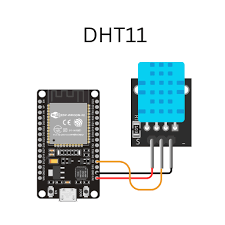
\includegraphics[width=1\linewidth]{Figuras/DHT11-ESP32.png}
    \end{figure}
    \end{column}
    \begin{column}{0.48\textwidth}
    \begin{itemize}
        \item Capabilities: Temperatura e umidade.
        \item Resource: ESP32
    \end{itemize}
    \end{column}

\end{columns}

\end{frame}

\begin{frame}{Exemplo: Xenotransplante}
    \begin{itemize}
        \item Criação de porcos para desenvolvimento de orgão para transplantes
        \item Queremos \textbf{acompanhar o peso} dos porcos
        \item Usamos uma balança para pesar todos os porcos
    \end{itemize}
    \vspace{1cm}
    \pause
    \begin{itemize}
        \item Capabilities: Peso
        \item Resources: Porcos
    \end{itemize}
\end{frame}

\begin{frame}{Arquitetura de microsserviços}
\begin{itemize}
    \item Separa um grande sistema em partes modulares, chamadas de \textbf{microsserviços}
    \item Cada microsserviço é independente dos demais.
    \item Os microsserviços se comunicam via rede (API REST em HTTP ou gRPC)
\end{itemize}
\end{frame}

\begin{frame}{Arquitetura de microsserviços}
\begin{figure}
    \centering
    \scalebox{.6}{
    \includesvg{ibira-arch}
    }
\end{figure}
\end{frame}



\section{Demonstração Prática}
\begin{frame}{Exercício}
\begin{itemize}
    \item  Acessar plataforma
    \item  Criar uma conta para cada pessoa/grupo
    \item  Registrar capabilities e resources
    \begin{itemize}
        \item Fazer um script (Python, bash, powershell) que mande dados para a plataforma
        \item Programar o ESP32 para mandar dados
    \end{itemize}
\end{itemize}
\begin{figure}
    \centering
    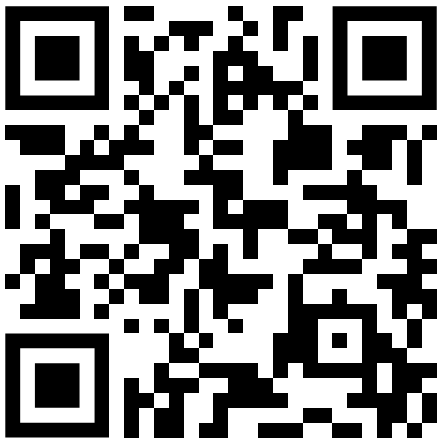
\includegraphics[width=0.3\linewidth]{QR-code-aula-mestrado.png}
    \caption{https://github.com/arthuript/Aula-plataformas-IoT}
\end{figure}
\end{frame}

\end{document}